\subsection{EndoWrist roll measurement}% \label{app:...}
The test setup for this measurement can be seen on \todo{figref and a picture below}

\subsection*{Test equipment:}
\begin{itemize}
\item Endowrist model 420093 (AAU number: \#4).
\item Maxon 110160 motor with attached Maxon gearhead 110356 and Maxon encoder 201937.
\item Torque sensor - Holger clasen: MWA-W8-1-P (AAU number: LBNR 08931).
\item Active low pass filter set to 100 Hz and gain 1 (AAU number: C2-104-H1).
\item Agilent 54621A oscilloscope (AAU number: 56684)
\end{itemize}

\subsection*{Procedure:}
The following procedure was made for the push force measurements:
\begin{enumerate}
\item The carbon stick of the EndoWrist is attached to the torque sensor. 
\item The torque sensor is connected to the low pass filter and the low pass filter to the oscilloscope.
\item Current is applied or increased to the motor which control the roll of the end-effector, with different current steps and the output from the torque sensor is noted.
\item Current is increased until 1200 mA is applied.
\end{enumerate}
Step three and four is repeated four times, where the current and torque is noted in respect to each other.. 
\todo{update n times}

\subsection*{Measuring data:}
The data from the measurements can be seen on \todo{Picture}

% This file was created by matlab2tikz.
%
%The latest updates can be retrieved from
%  http://www.mathworks.com/matlabcentral/fileexchange/22022-matlab2tikz-matlab2tikz
%where you can also make suggestions and rate matlab2tikz.
%
\definecolor{mycolor1}{rgb}{0.00000,0.44700,0.74100}%
\definecolor{mycolor2}{rgb}{0.85000,0.32500,0.09800}%
\definecolor{mycolor3}{rgb}{0.92900,0.69400,0.12500}%
\definecolor{mycolor4}{rgb}{0.49400,0.18400,0.55600}%
%
\begin{figure}
\begin{tikzpicture}

\begin{axis}[%
width=4.521in,
height=3.566in,
at={(0.758in,0.481in)},
scale only axis,
xmin=0,
xmax=1.2,
xlabel style={font=\color{white!15!black}},
xlabel={Curremt [A]},
ymin=0,
ymax=9,
ylabel style={font=\color{white!15!black}},
ylabel={Torque [Ncm]},
axis background/.style={fill=white},
title style={font=\bfseries},
title={Relation between roll force and ampere}
]
\addplot [color=mycolor1, draw=none, mark=asterisk, mark options={solid, mycolor1}, forget plot]
  table[row sep=crcr]{%
0.063	0.34\\
0.097	0.4\\
0.125	0.6\\
0.16	0.8\\
0.208	1.1\\
0.241	1.32\\
0.3	1.86\\
0.38	2.1\\
0.73	4.7\\
1.02	6.68\\
};
\addplot [color=mycolor2, draw=none, mark=asterisk, mark options={solid, mycolor2}, forget plot]
  table[row sep=crcr]{%
0.06	0.7\\
0.12	0.72\\
0.175	0.9\\
0.24	1.54\\
0.3	2\\
0.37	2.42\\
0.42	2.88\\
0.489	3.26\\
0.568	4\\
0.73	4.98\\
0.876	6\\
1.12	7.5\\
};
\addplot [color=mycolor3, draw=none, mark=asterisk, mark options={solid, mycolor3}, forget plot]
  table[row sep=crcr]{%
0.03	0.04\\
0.06	0.8\\
0.276	2.02\\
0.42	3.06\\
0.568	4.24\\
0.73	5.24\\
0.877	6.48\\
1.02	7.28\\
};
\addplot [color=mycolor4, draw=none, mark=asterisk, mark options={solid, mycolor4}, forget plot]
  table[row sep=crcr]{%
0.064	1.2\\
0.16	1.38\\
0.275	2.12\\
0.389	2.86\\
0.51	3.84\\
0.631	4.82\\
0.78	5.7\\
0.94	7.06\\
1.12	8.1\\
};
\end{axis}
\end{tikzpicture}%
\caption{Torque measurements of the roll on the EndoWrist.}
\label{fig:torque_measurement}
\end{figure}

%\figref{endo_force_mes}. 
%\eqref{eq:linear_force_endo}.

% \begin{equation}
% \text{y} = 0.0028 \cdot \text{x} -0.8259 
% \label{eq:linear_force_endo}
% \end{equation} 



\subsection*{Results:}
\todo{result}


%It can be seen from the graph on \figref{endo_force_mes} that the force on the end-effector is highly nonlinear. The friction from the gearing and the Endowrist does that the force first has an exponential growth at the start. Around the 800 mA and 1200 mA step it can be seen that a drop in force is happening. What causes this drop is not identified but it can be seen that it appears for all the data sequences. \todor{better explanation?}


%% This file was created by matlab2tikz.
%
%The latest updates can be retrieved from
%  http://www.mathworks.com/matlabcentral/fileexchange/22022-matlab2tikz-matlab2tikz
%where you can also make suggestions and rate matlab2tikz.
%
\definecolor{mycolor1}{rgb}{0.00000,0.44700,0.74100}%
\definecolor{mycolor2}{rgb}{0.85000,0.32500,0.09800}%
%
\begin{figure}[h]
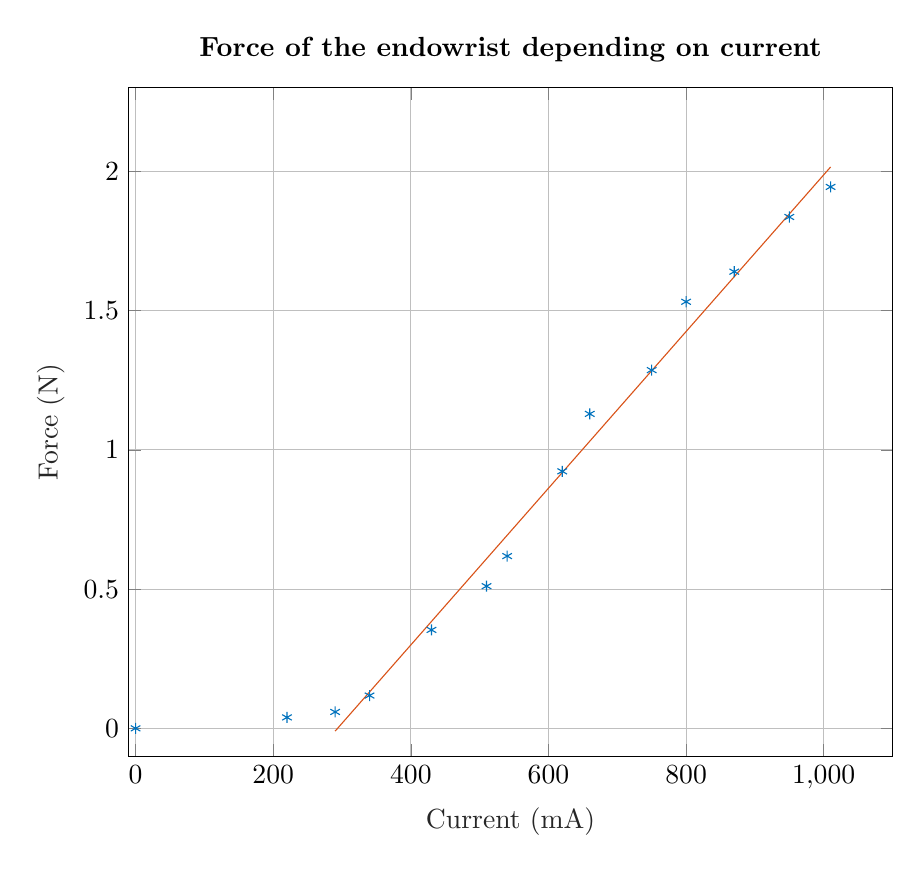
\begin{tikzpicture}

\begin{axis}[%
width=0.8\columnwidth,%7.484in,
height=0.7\columnwidth,%8.26in,
at={(0.758in,0.481in)},
scale only axis,
xmin=-10,
xmax=1100,
xlabel style={font=\color{white!15!black}},
xlabel={Current (mA)},
ymin=-0.1,
ymax=2.3,
ylabel style={font=\color{white!15!black}},
ylabel={Force (N)},
axis background/.style={fill=white},
title style={font=\bfseries},
title={Force of the endowrist depending on current},
xmajorgrids,
ymajorgrids
]
\addplot [color=mycolor1, draw=none, mark=asterisk, mark options={solid, mycolor1}, forget plot]
  table[row sep=crcr]{%
0	0\\
220	0.03928\\
290	0.05892\\
340	0.11784\\
430	0.35352\\
510	0.51064\\
540	0.61866\\
620	0.92308\\
660	1.1293\\
750	1.28642\\
800	1.53192\\
870	1.63994\\
950	1.83634\\
1010	1.94436\\
};
\addplot [color=mycolor2, forget plot]
  table[row sep=crcr]{%
290	-0.00996204344902341\\
340	0.130719594329395\\
430	0.383946542330548\\
510	0.609037162776017\\
540	0.693446145443068\\
620	0.918536765888537\\
660	1.03108207611127\\
750	1.28430902411242\\
800	1.42499066189084\\
870	1.62194495478063\\
950	1.8470355752261\\
1010	2.0158535405602\\
};
\end{axis}
\end{tikzpicture}%
\caption{The force measurements from the end-effector}
\label{endo_force_mes}
\end{figure}

\subsection*{Uncertainties of measurement:}
\begin{itemize}
\item Gain of low pass filter could deviate from 1.
\end{itemize}

\subsection*{Conclusion:}
It can be seen on figure \figref{fig:torque_measurement} that the roll-torque of the EndoWrist has a linear growth from approx. 100 mA and up. The parameters for this estimation can therefore be expressed as y = A$\cdot$x+B.

